%\documentclass{beamer}
\documentclass[handout]{beamer}
\usetheme{Marburg}
\useoutertheme{infolines}
\newcommand{\answers}{1}

\usepackage{amsmath}
\usepackage{caption}
\usepackage{color}
\usepackage{enumerate}
\usepackage{listings}
\usepackage{hyperref}
\usepackage{mathrsfs}
\usepackage{natbib}
\usepackage{url}

\providecommand{\all}{\ \forall \ }
\providecommand{\bs}{\backslash}
\providecommand{\e}{\varepsilon}
\providecommand{\E}{\ \exists \ }
\providecommand{\lm}[2]{\lim_{#1 \rightarrow #2}}
\providecommand{\m}[1]{\mathbb{#1}}
\providecommand{\nv}{{}^{-1}}
\providecommand{\ov}[1]{\overline{#1}}
\providecommand{\p}{\newpage}
\providecommand{\q}{$\quad$ \newline}
\providecommand{\rt}{\rightarrow}
\providecommand{\Rt}{\Rightarrow}
\providecommand{\vc}[1]{\boldsymbol{#1}}
\providecommand{\wh}[1]{\widehat{#1}}

\hypersetup{colorlinks,linkcolor=,urlcolor=blue}
\numberwithin{equation}{section}

\definecolor{dkgreen}{rgb}{0,0.6,0}
\definecolor{gray}{rgb}{0.5,0.5,0.5}
\definecolor{mauve}{rgb}{0.58,0,0.82}

\lstset{ 
  language=C,                % the language of the code
  basicstyle= \footnotesize,           % the size of the fonts that are used for the code
  numbers=left,
  numberfirstline=true,
  numbersep=5pt,                  % how far the line-numbers are from the code
  backgroundcolor=\color{white},      % choose the background color. You must add \usepackage{color}
  showspaces=false,               % show spaces adding particular underscores
  showstringspaces=false,         % underline spaces within strings
  showtabs=false,                 % show tabs within strings adding particular underscores
  frame=lrb,                   % adds a frame around the code
  rulecolor=\color{black},        % if not set, the frame-color may be changed on line-breaks within not-black text 
  tabsize=2,                      % sets default tabsize to 2 spaces
  captionpos=t,                   % sets the caption-position 
  breaklines=true,                % sets automatic line breaking
  breakatwhitespace=false,        % sets if automatic breaks should only happen at whitespace
  %title=\lstname,                   % show the filename of files included with \lstinputlisting;
  keywordstyle=\color{blue},          % keyword style
  commentstyle=\color{gray},       % comment style
  stringstyle=\color{dkgreen},         % string literal style
  escapeinside={\%*}{*)},            % if you want to add LaTeX within your code
  morekeywords={*, ...},               % if you want to add more keywords to the set
  xleftmargin=0.2in, % left horizontal offset of caption box
  xrightmargin=-.03in % right horizontal offset of caption box
}

%\DeclareCaptionFont{white}{\color{white}}
%\DeclareCaptionFormat{listing}{\parbox{\textwidth}{\colorbox{gray}{\parbox{\textwidth}{#1#2#3}}\vskip-0.05in}}
%\captionsetup[lstlisting]{format = listing, labelfont = white, textfont = white}
%For caption-free listings, comment out the 3 lines above and uncomment the 2 lines below.
 \captionsetup{labelformat = empty, labelsep = none}
 \lstset{frame = single}

\title{Introduction to GPU computing for statisticicans}
\author{Will Landau}
\date{September 16, 2013}
\institute{Iowa State University}

\begin{document}

\begin{frame}
\titlepage
 \end{frame}
 
\begin{frame}
\frametitle{Outline}
\tableofcontents
\end{frame} 
 
 \AtBeginSection[]
{
   \begin{frame}
       \frametitle{Outline}
       \tableofcontents[currentsection]
   \end{frame}
}

\section{GPUs, parallelism, and why we care}

\begin{frame}[fragile]
\frametitle{The single instruction, multiple data (SIMD) paradigm}

\begin{itemize}
\pause \item SIMD: apply the same command to multiple places in a dataset. 

\pause \begin{lstlisting}
for(i = 0; i < 1e6; ++i)
  a[i] = b[i] + c[i];
\end{lstlisting}


\pause \item On CPUs, the iterations of the loop run sequentially.

\pause \item With GPUs, we can easily run all 1,000,000 iterations simultaneously.

\pause \begin{lstlisting}
i = threadIdx.x;
a[i] = b[i] + c[i];
\end{lstlisting}

\pause \item We can similarly \emph{parallelize} a lot more than just loops.
\end{itemize}
\end{frame}





\begin{frame}
\frametitle{Parallel MCMC by Lee, Yau, Giles, and others}

\scriptsize
\begin{center}
\begin{tabular}{llll}
\# chains & CPU time (min) & GTX 280 (min) & CPU time / GPU time \\ \hline
8 & 0.0166 & 0.0148 & 1.1 \\
32 & 0.0656 & 0.0151 & 4 \\
128 & 0.262 & .0154 & 17 \\
512 & 1.04 & 0.0174  & 60 \\
2,048 & 4.16 & 0.0248 & 168 \\
8,192 & 16.64 & 0.0720 & 230 \\
32,768 & 66.7 & 0.249 & 268 \\
131,072 & 270.3 & 0.970 & 279
\end{tabular}
\end{center}

\end{frame}



\begin{frame}
\frametitle{Parallel sequential MC by Lee, Yau, Giles, and others}


\scriptsize
\begin{center}
\begin{tabular}{llll}
Sample size & CPU time (min) & GTX 280 (min) & CPU time / GPU time \\ \hline
8,192 & 4.44 & 0.0199 & 223.1 \\
16,384 & 8.82 & 0.0355 & 263 \\
32,768 & 17.7 & 0.0666 & 265 \\
65,536 & 35.3 & 0.131 & 269 \\
131,076 & 70.6 & 0.261 & 270.5 \\
262,144 & 141 & 0.52 & 271.2
\end{tabular}
\end{center}
\end{frame}

\begin{frame}
\frametitle{Parallel Bayesian EM by Suchard, Wang, Chan, and others}

\scriptsize
\begin{center}
\begin{tabular}{llll}
Sample size & cpu 1 (sec) & gpu 1 (sec) & CPU time / GPU Time \\ \hline
$10^2$ & 4.0 & 71.1 & 0.1 \\
$10^3$ & 40.0 &  81.3  & 0.5 \\
$10^4$ & 607.0 & 91.2  & 6.7 \\
$10^5$ & 7793.0 & 129.6  & 60.1 \\
$10^6$ & 78765.0 & 680.6  & 115.7 \\
\end{tabular}
\end{center}

\end{frame}




\begin{frame}
\frametitle{Other applications}
\begin{itemize}
\item Clustering
\pause \item Bootstrap
\pause \item Regression
\pause \item Matrix algebra
\pause \item EM Algorithm
\pause \item Rejection sampling 
\pause \item Multiple testing
\pause \item Cross validation
\item $\cdots$
\end{itemize}

\end{frame}

\begin{frame}
\frametitle{Computer processors}
\begin{itemize}
\item {\bf Processing unit}: a computer chip that performs executive functions. 
\pause \item {\bf Core}: One of possibly many ``sub-processors" placed on the same processing unit, each of which has the full functionality of the processing unit.
\end{itemize}

\end{frame}


\begin{frame}
\frametitle{The Central Processing Unit (CPU)}

\begin{itemize}
\item Regular computer processor.
\pause \item Allows parallelism, but not \emph{massive} parallelism on its own.
\pause \item Usually contains 1 to 8 cores.
\pause \item Examples:
\begin{itemize}
\item Intel 8086 (1979, x86)
\pause \item Intel Core 2 Duo
\pause \item  Intel 80486DX2 (below)
\end{itemize}
\end{itemize}

\begin{center}
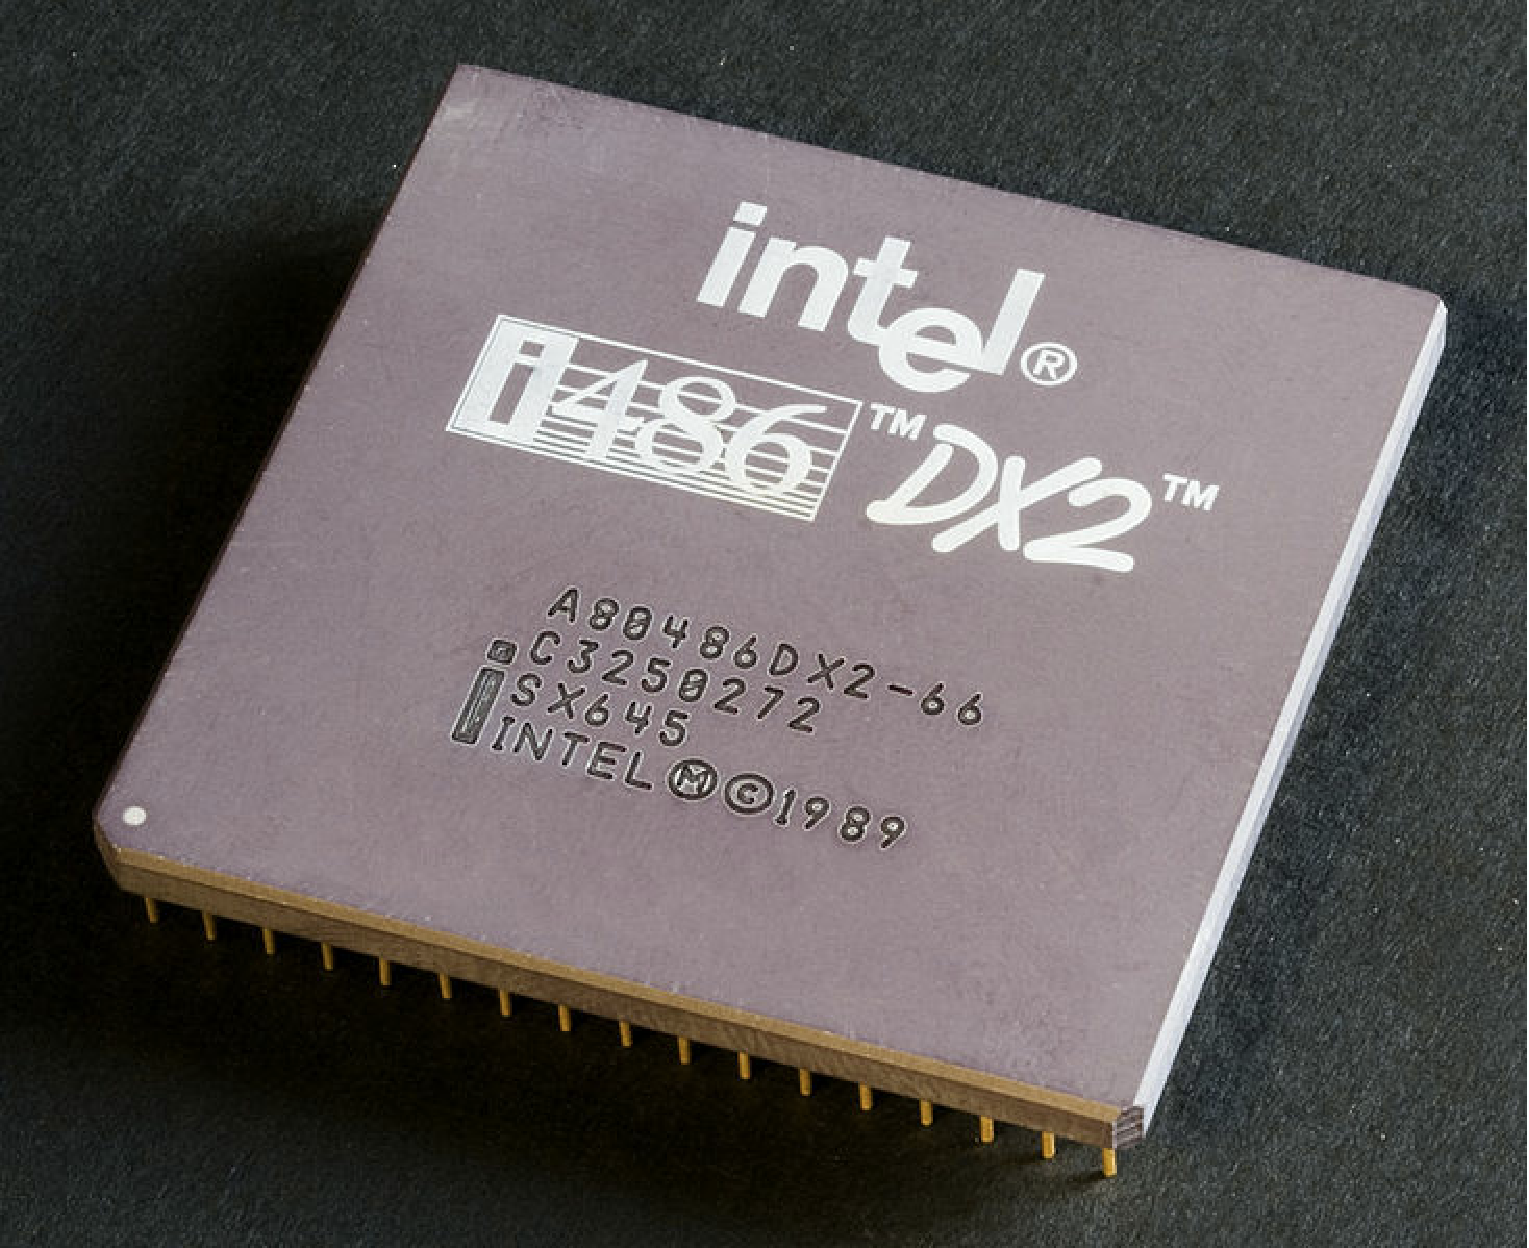
\includegraphics[scale = .175, angle = -1]{../../fig/cpu1} $\quad$ 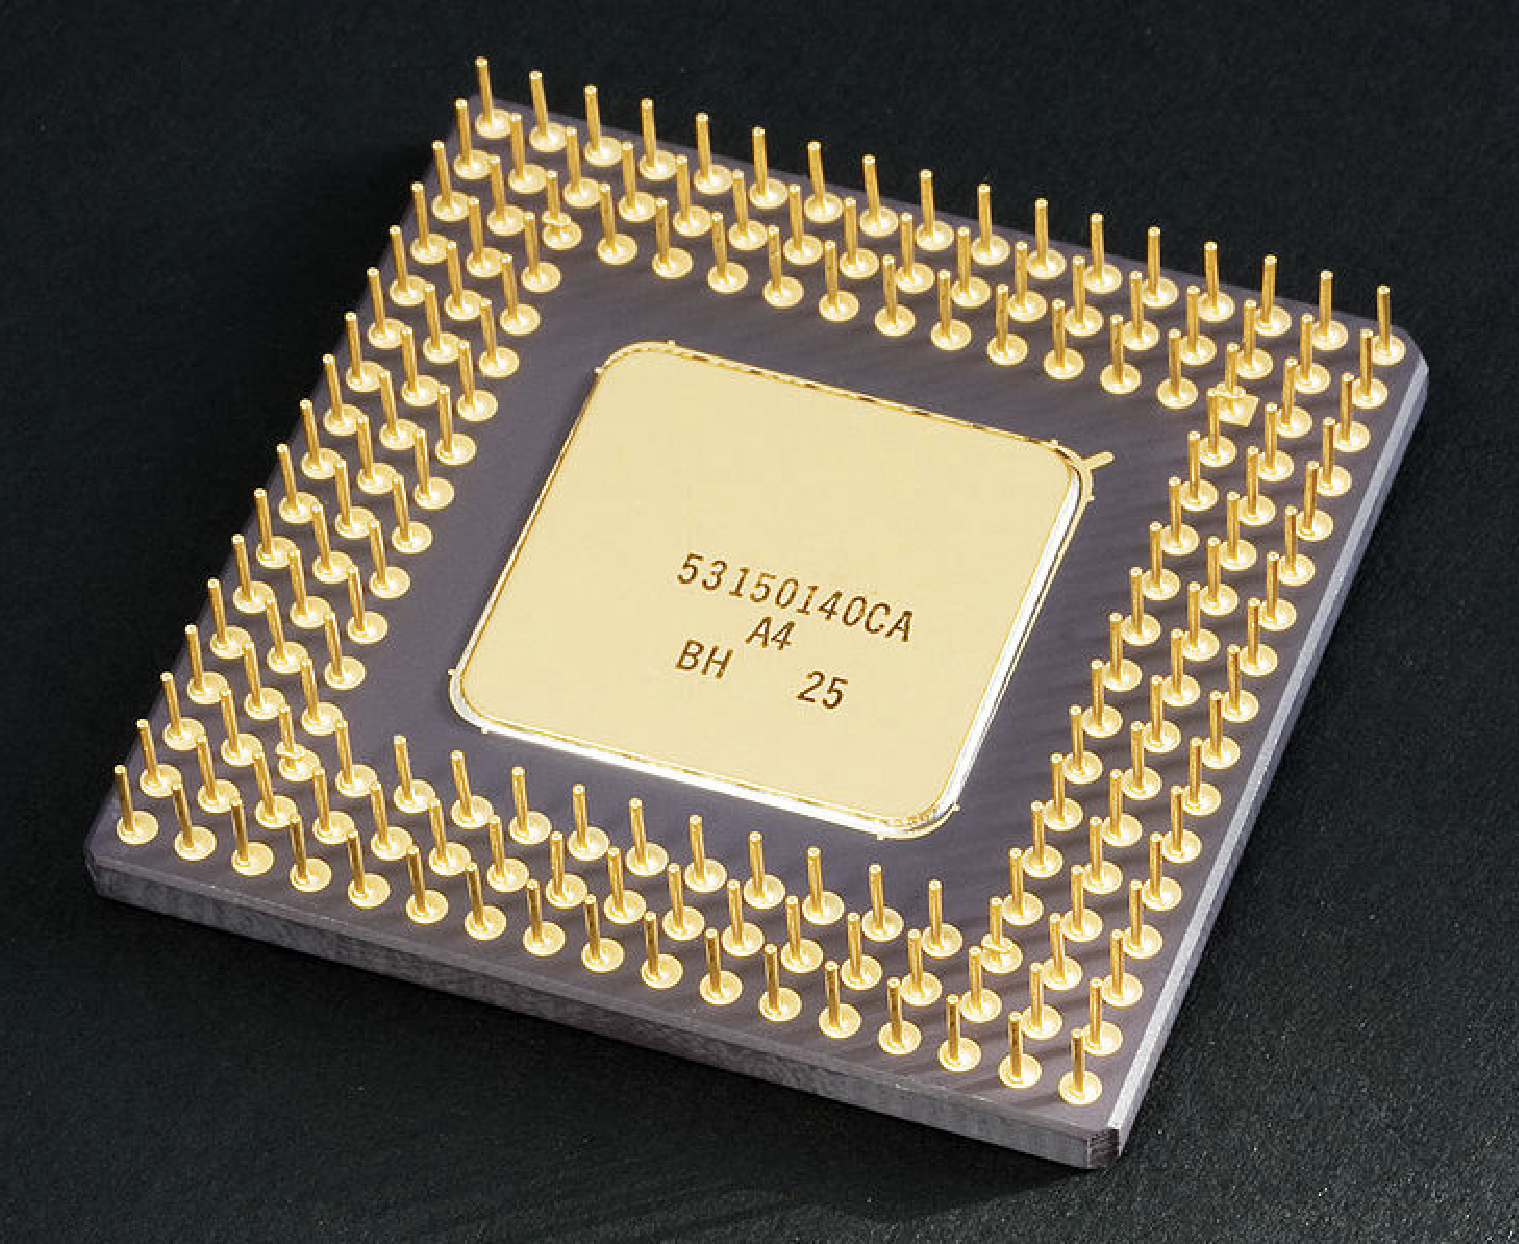
\includegraphics[scale = .175, angle = -1]{../../fig/cpu2}
\end{center}
\end{frame}



\begin{frame}
\frametitle{The Graphics Processing Unit (GPU)}
\scriptsize

\begin{itemize}\scriptsize
\item Processor in a video card or graphics card.
\pause \item Massively parallel: originally designed to speed up graphics throughput in video games.
\pause \item Cannot run by itself. Needs to be hooked up to a computer with a CPU.
\pause \item Contains several hundred cores.
\pause \item Higher memory bandwidth than a CPU.
\pause \item Examples:
\begin{itemize}\scriptsize
\item NVIDIA GeForce 6600 (bottom left)
\pause \item NVIDIA GeForce GTX 580 
\pause \item NVIDIA Tesla M2070 (on our GPU-enabled machines)
\end{itemize}

\end{itemize}

\begin{center}
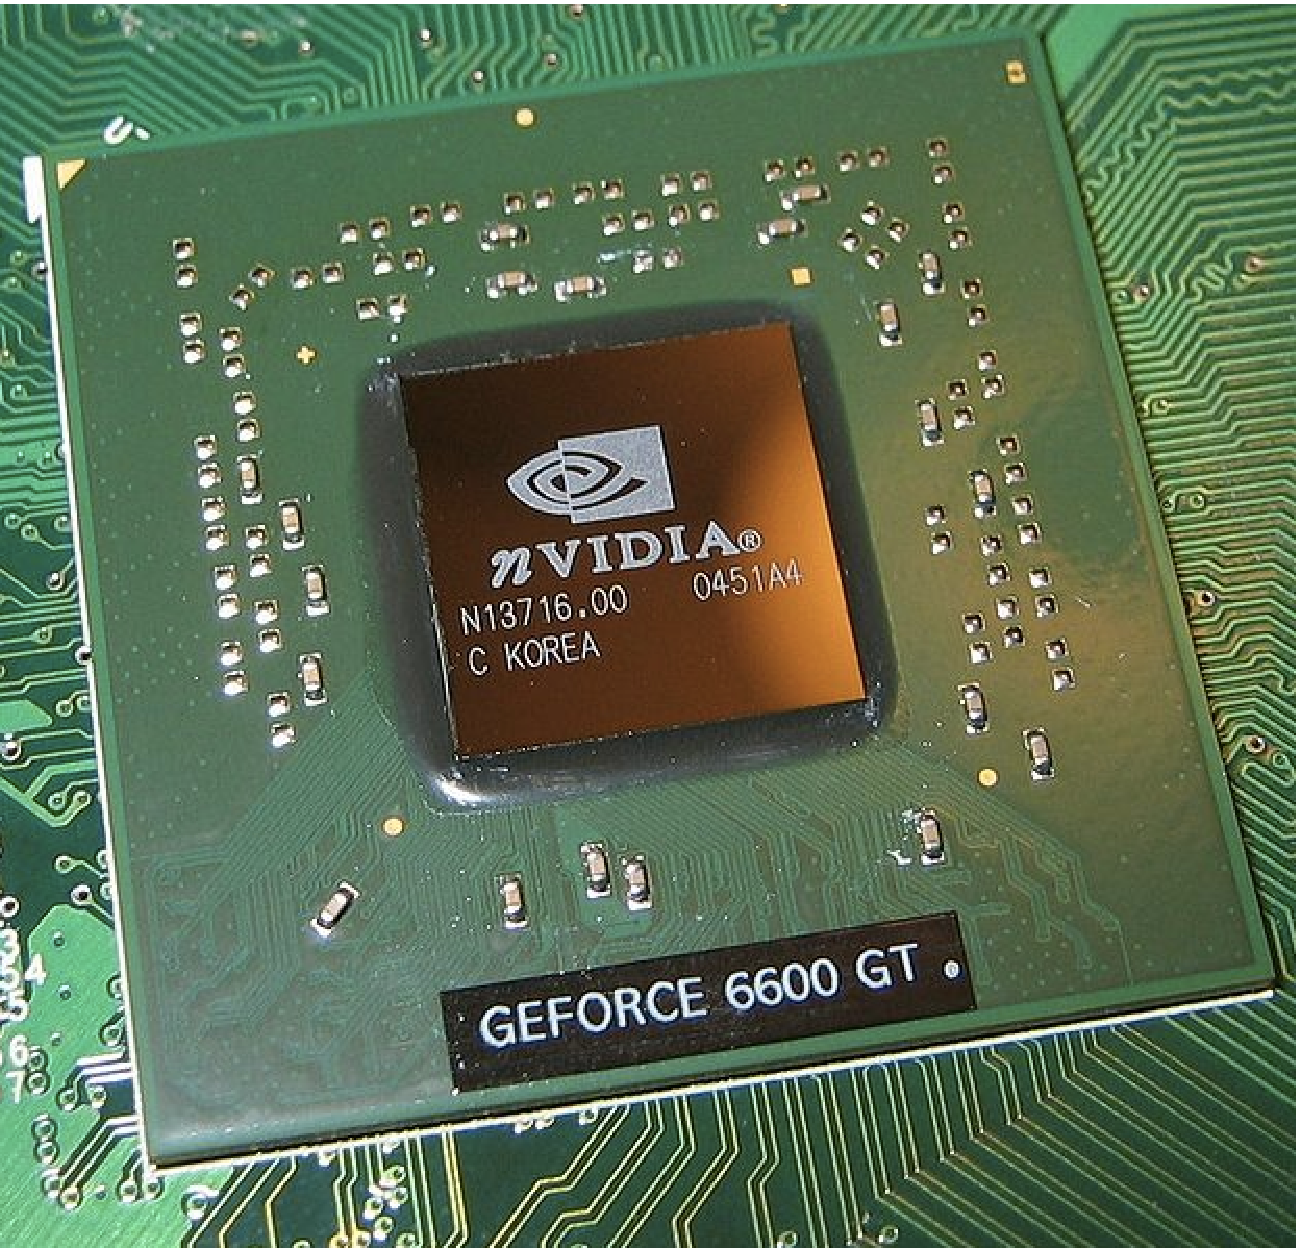
\includegraphics[scale = .175]{../../fig/gpu1} $\quad$ 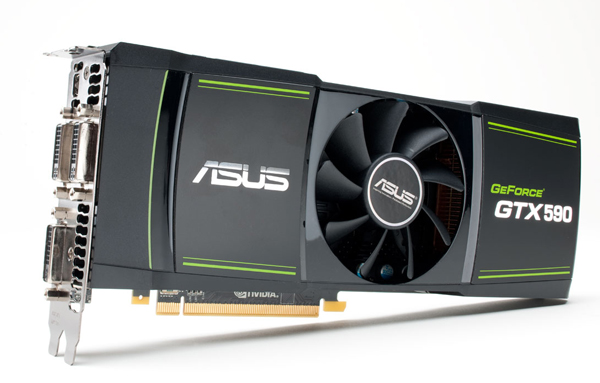
\includegraphics[scale = .175]{../../fig/gpu2}
\end{center}

\end{frame}


\begin{frame}
\frametitle{CPU / GPU cooperation}

\begin{itemize}
\item The CPU (``host") is in charge.
\uncover<2->{\item The CPU sends computationally intensive instruction sets to the GPU (``device") just like a human uses a pocket calculator.}
\end{itemize}

\begin{center}
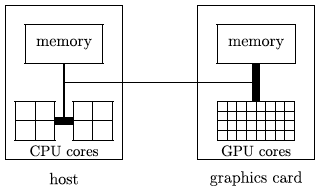
\includegraphics[scale=.8]{../../fig/communication.png}
\end{center}
\end{frame}

\begin{frame}
\frametitle{More on parallelism}
\begin{itemize}
\item {\bf Parallelism}: the practice of running multiple calculations simultaneously.
\pause \item The architecture of GPUs is extremely well-suited to massively parallel workflows.
\pause \item Note: GPU parallelism is one of many kinds of parallelism. Others include:
\begin{itemize}
\pause \item Posix threads (CPU parallelism)
\pause \item parallel cloud computing
\pause \item openMP parallelism
\pause \item openMP parallelism
\end{itemize}
\end{itemize}
\end{frame}

\begin{frame}
\frametitle{GPU parallelism speeds up calculations}
\begin{itemize}
\item Amdahl's Law says that the maximum theoretical speedup (CPU time / GPU time) is
\pause \begin{align*}
\frac{1}{1 - P + \frac{P}{N}}
\end{align*}
where:
\begin{itemize}
\item $P$ = fraction of the program (in terms of execution time) that can be parallelized
\item $N$ = number of parallel processors
\end{itemize}
\pause \item As $N \rt \infty$, Amdahl's quantity goes to
\begin{align*}
\frac{1}{1 - P}
\end{align*}
\pause \item So if 99\% of the program can be parallelized, we could theoretically have a 100-fold speedup.
\end{itemize}
\end{frame}



\begin{frame}
\frametitle{How GPU parallelism works} \scriptsize
\begin{enumerate}
\scriptsize
\item The CPU sends a command called a {\bf kernel} to a GPU.
\pause \item The GPU executes several duplicate realizations of this command, called {\bf threads}.
\begin{itemize}
\scriptsize
\pause \item These threads are grouped into bunches called {\bf blocks}.
\pause \item The sum total of all threads in a kernel is called a {\bf grid}.
\end{itemize}
\end{enumerate}

\begin{itemize}
\scriptsize
\item Toy example:
\begin{itemize}
\scriptsize
\item CPU says something like, ``Hey, GPU. Sum pairs of adjacent numbers. Use the array, (1, 2, 3, 4, 5, 6, 7, 8). Use 2 blocks of 2 threads each."
\pause \item GPU thinks: ``Sum pairs of adjacent numbers" is a kernel that I need to apply to the array, (1, 2, 3, 4, 5, 6, 8).
\pause \item The GPU spawns 2 blocks, each with 2 threads:
\end{itemize}
\end{itemize}

\pause \begin{center}
\begin{tabular}{c|cc|cc}
Block  & \multicolumn{2}{c|}{0} &  \multicolumn{2}{c}{1} \\ \hline
Thread & 0 & 1 & 0 & 1  \\ \hline
Action & 1 + 2 & 3 + 4 & 5 + 6 & 7 + 8 \\
\end{tabular}
\end{center}

\begin{itemize}
\scriptsize
\pause \item All four actions above happen simultaneously.
\pause \item I could have also used 1 block with 4 threads and given the threads different paris of numbers.
\end{itemize}
\end{frame}

\begin{frame}
\begin{center}
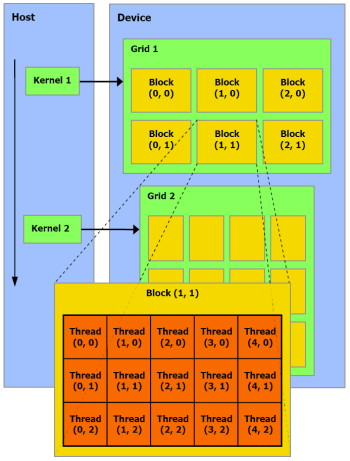
\includegraphics[scale=.7]{../../fig/gridBlocksThreads.jpg}
\end{center}
\end{frame}



\section{CUDA and our CUDA systems}

\begin{frame}
\frametitle{CUDA: making a gaming toy do science}
\begin{itemize}
 \item GPUs were originally meant to speed up graphical displays for Windows OS and video games.
 \end{itemize}
 \begin{center}
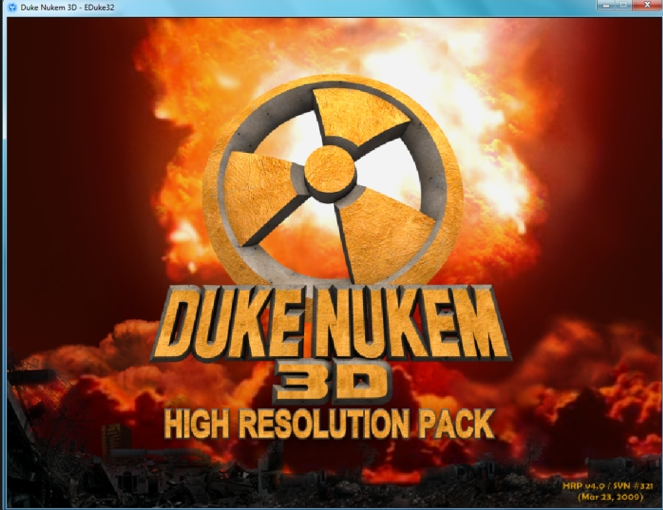
\includegraphics[scale=.19]{../../fig/nukem.png}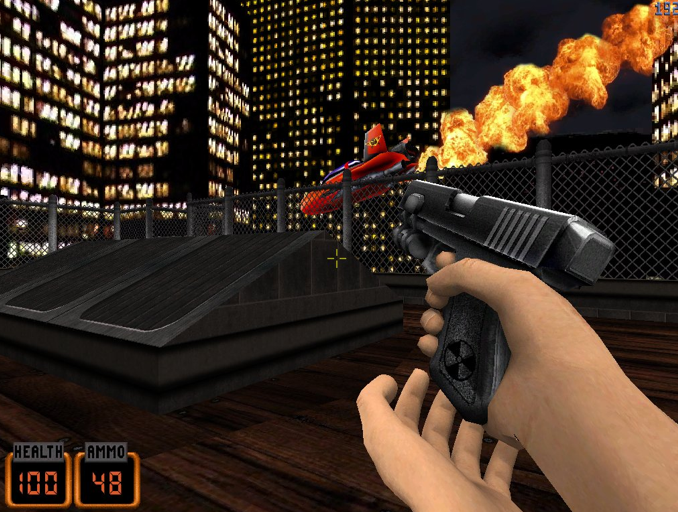
\includegraphics[scale=.19]{../../fig/nukem2.png}
\end{center}
\begin{itemize}
\pause \item {\bf CUDA}: Compute Unified Device Architecture. 
\pause \item Before CUDA, programmers could only program on GPUs using graphics languages, which are appropriate for video games but clumsy for science.
\pause \item CUDA devices support CUDA C, an extension of C for programs that use GPUs.
\end{itemize}
\end{frame}

\begin{frame}
\frametitle{CUDA-enabled servers at Iowa State}
\begin{itemize}
\item impact1.stat.iastate.edu (Red Hat Enterprise Linux Server release 6.2)
\item impact2.stat.iastate.edu (CentOS release 6.3)
\item impact3.stat.iastate.edu (Red Hat Enterprise Linux Server release 6.4)
\item impact4.stat.iastate.edu (CentOS release 6.4)
\end{itemize}
\end{frame}


\begin{frame}[fragile]
\frametitle{Specs of our CUDA systems}
\begin{itemize}
\item No graphical user interface or remote desktop capabilities. (Use the Linux command line.)
\pause \item 24 CPUs and 4 Tesla M2070 GPUs, where each GPU has 448 cores.:
\pause \item For more specs, log into impact1, 2, or 3 and enter into the command line:
\begin{lstlisting}
cd /usr/local/NVIDIA_GPU_Computing_SDK/C/bin/linux/release
./deviceQuery
\end{lstlisting}
\end{itemize}
\end{frame}

\begin{frame}[fragile]
\frametitle{Logging in}
\small 

\begin{itemize}
\item Open a command line program (Terminal in Linux and Mac OS, Cygwin or MinGW in Windows).
\pause \item Enter:
\begin{lstlisting}
ssh -p 323 ISU_ID@impact1.stat.iastate.edu
\end{lstlisting}
\pause \item Note: in general, the port number for {\tt ssh} is not always 323.
\pause \item Refer to \url{http://www.linuxcommand.org/} or contact me at landau@iastate.edu for help with the Linux command line.
\pause \item Contact Stat IT at statit@iastate.edu or me if:
\begin{itemize}
\pause \item You can't log on, or
\pause \item You want to be able to log on without entering your password every time, or
\pause \item You want to shorten {\tt ssh -p 323 ISU\_ID@impact1.stat.iastate.edu} into a more manageable alias on your local machine.
\end{itemize}
\end{itemize}
\end{frame}

\begin{frame}
\frametitle{Important directories} \small
\begin{itemize}
\item {\bf /home/ISU\_ID} Your private home folder on SMB (the collective storage system for all the stat dept linux servers). Files in here are stored remotely on SMB, not locally on impact1-3.
\pause \item {\bf /Cyfiles/ISU\_ID} Your private Cyfiles folder. Files in here are stored remotely on the Cyfiles server, not locally on impact1-3.
\pause \item {\bf /tmp} 
\begin{itemize}
\item Everything in here is stored locally on impact1, etc., wherever you're logged in.  
\pause \item To avoid communicating over a network when you want fast computation, put large datasets here.
\pause \item Note: {\bf /tmp} automatically empties periodically.
\end{itemize}
\pause \item {\bf /usr/local/NVIDIA\_GPU\_Computing\_SDK}
\begin{itemize}
\item Example CUDA C code. Stored locally on impact1, etc.
\pause \item You do not have write privileges here.
\end{itemize}
\end{itemize}
\end{frame}


\section{GPU computing with R}


\begin{frame}
\frametitle{GPU-enabled R packages}
\begin{itemize}
\item {\tt WideLM} - used to quickly fit a large number of linear models to a fixed design matrix and response vector.
\pause \item {\tt magma} - a small linear algebra with implementations of backsolving and the LU factorization.
\pause \item {\tt cudaBayesreg} - implements a Bayesian model for fitting fMRI data.
\pause \item  {\tt gcbd} - a Debian package for �benchmarking� linear algebra algorithms such as the QR, SVD and LU.factorizations.
\pause \item {\tt gputools} - probably the most useful of these 5.
\end{itemize}
\end{frame}



\begin{frame}
\frametitle{Contents of {\tt gputools}}


\begin{itemize}
\item Choose your device:

\begin{center}
\begin{tabular}{r|l|c}
 \bf gputools function & \bf CPU analog  & \bf Same usage? \\ \hline
chooseGpu() & none & NA \\
getGpuId() & none & NA
\end{tabular}
\end{center}

\pause \item Linear algebra: 
\begin{center}
\begin{tabular}{r|l|c}

 \bf gputools function & \bf CPU analog  & \bf Same usage? \\ \hline
gpuDist() & dist() & no \\ 
gpuMatMult() & \%*\% operator & no \\ 
gpuCrossprod() & crossprod() & yes \\ 
gpuTcrossprod() & tcrossprod() & yes \\ 
gpuQr() & qr() & almost \\ 
gpuSolve() & solve() & no \\ 
gpuSvd() & svd() & almost \\ 
\end{tabular}
\end{center}
\end{itemize}
\end{frame}


\begin{frame}
\begin{itemize}
\item Simple model fitting: 
\begin{center}
\begin{tabular}{r|l|c}

 \bf gputools function & \bf CPU analog  & \bf Same usage? \\ \hline
gpuLm() & lm() & yes \\ 
gpuLsfit() & lsfit() & yes \\ 
gpuGlm() & glm() & yes \\
gpuGlm.fit() & glm.fit() & yes \\ 
\end{tabular} $\quad$ \newline
\end{center}

\pause \item Hypothesis testing: 

\begin{center}
\begin{tabular}{r|l|c}
 \bf gputools function & \bf CPU analog  & \bf Same usage? \\ \hline
gpuTtest() & t.test() & no \\ 
getAucEstimate() & ??? & ??? \\
\end{tabular} $\quad$ \newline
\end{center}
\end{itemize}
\end{frame}



\begin{frame}
\begin{itemize}
\item Other routines: \scriptsize
\begin{center}
\begin{tabular}{r|l|c}
\bf gputools function & \bf CPU analog  & \bf Same usage? \\ \hline
gpuHclust() & hclust() & no \\
gpuDistClust() & hclust(dist()) & no \\ 
gpuFastICA() & fastICA() (fastICA package) & yes \\
gpuGranger() & grangertest() (lmtest package) & no \\
gpuMi() & ??? & ??? \\
gpuSvmPredict() & www.jstatsoft.org/v15/i09/paper & no \\
gpuSvmTrain() & www.jstatsoft.org/v15/i09/paper & no \\
\end{tabular}
\end{center}
\end{itemize}
\end{frame}




\begin{frame}[fragile]
\frametitle{Example}

\begin{lstlisting}
> getGpuID()
[1] 0
> chooseGpu(3)
[[1]]
[1] 3
> getGpuID()
[1] 3
> A <- matrix(runif(1e7), nrow = 1e4)
> B <- matrix(runif(1e7), nrow = 1e4)
> ptm <- proc.time(); C <- gpuMatMult(A, B); 
> proc.time() - ptm
   user   system  elapsed
   2.959  2.190     5.159
> ptm <-  proc.time(); C <- A % * % B; 
> proc.time() - ptm
   user   system  elapsed
   116.389  0.166   116.503
\end{lstlisting}
\end{frame}


\begin{frame}
\frametitle{Speedup}
\begin{center}
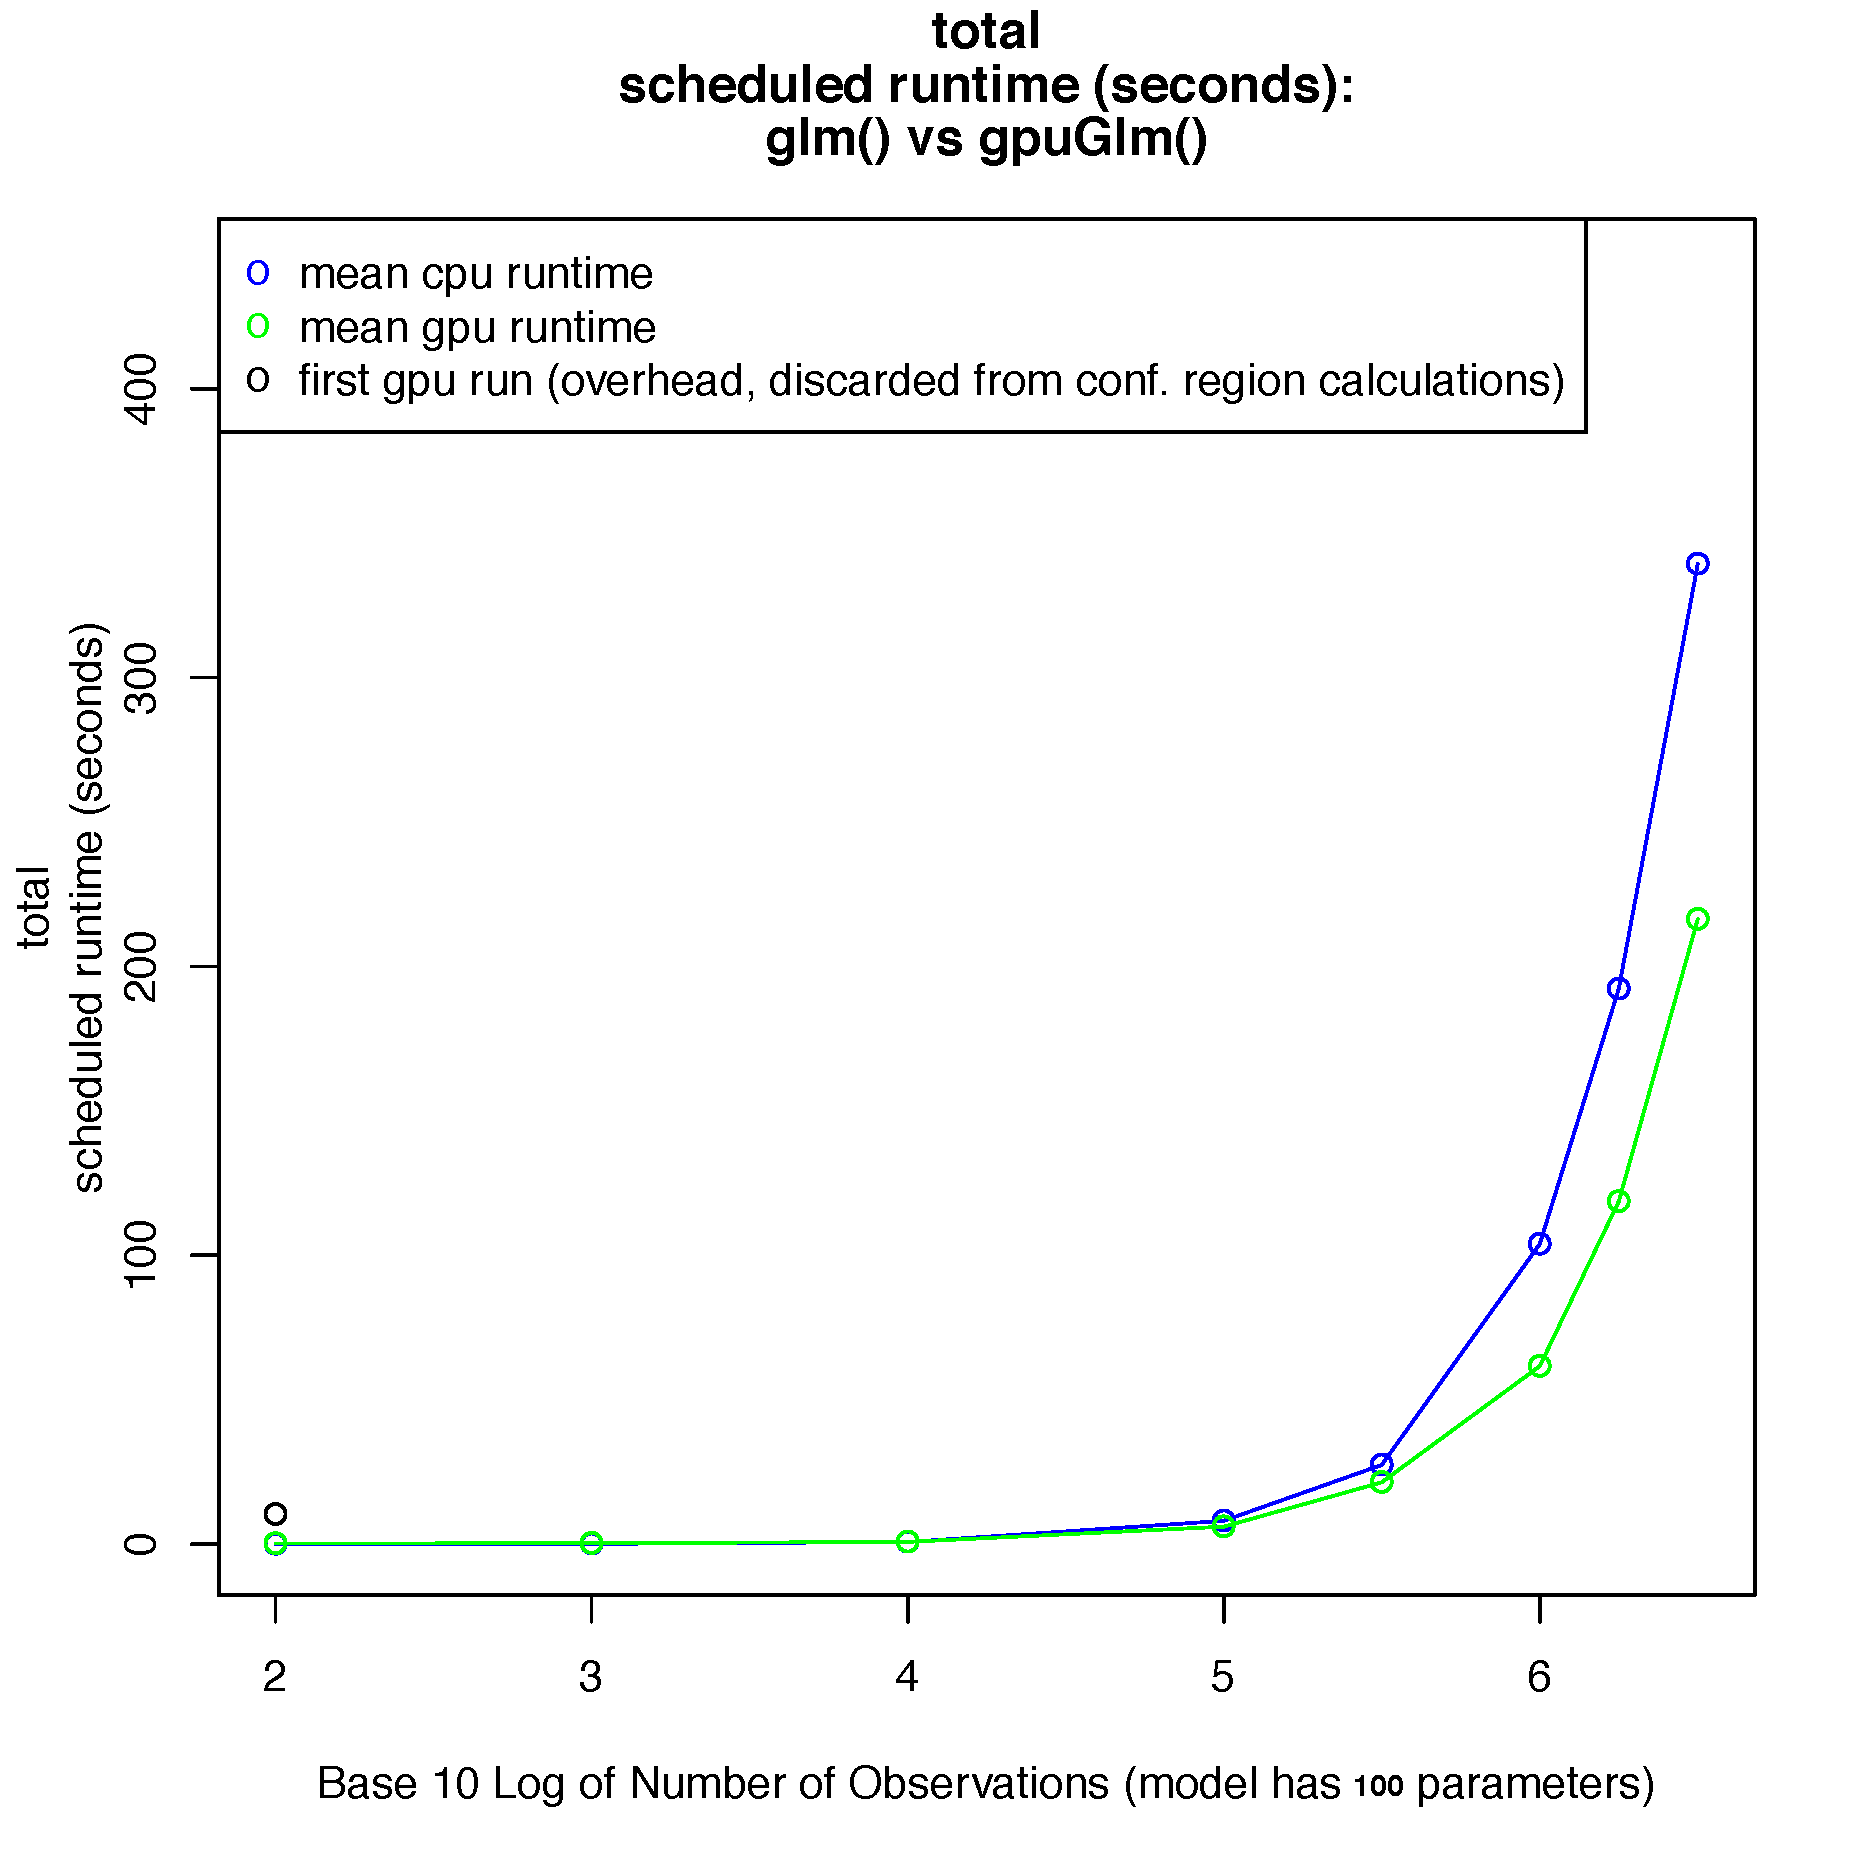
\includegraphics[scale=.25]{../../fig/gpuglm}
\end{center}
\end{frame}


\begin{frame}
\frametitle{Speedup}
\begin{center}
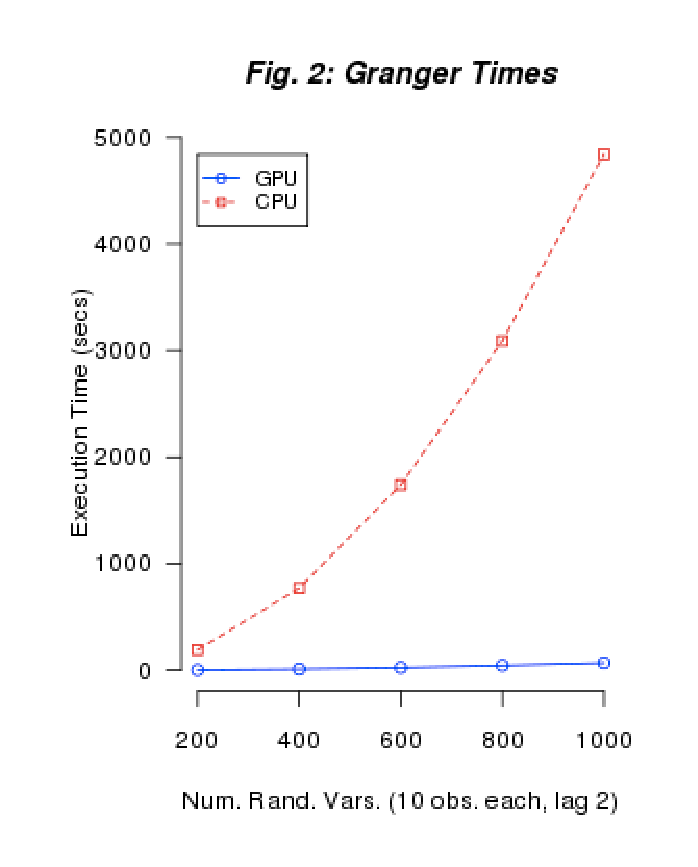
\includegraphics[scale=.55]{../../fig/granger}
\end{center}
\end{frame}

\begin{frame}
\frametitle{Tentative Syllabus}

\small
\begin{enumerate}
\item Intro and {\tt gputools}
\pause \item A codeless intro to GPU parallelism
\pause \item Intro to CUDA C
\pause \item CUDA C: K-means and MCMC
\pause \item CUDA C: Shared memory and performance measurement
\pause \item CUDA C: Race conditions, atomics, and warps
\pause \item CUBLAS and CULA: linear algebra libraries for CUDA C
\pause \item CURAND: a GPU-enabled library for fast random number generation
\pause \item Thrust: the GPU analog of the C++ Standard Template Library
\pause \item Intro to Python: preparation for PyCUDA
\pause \item PyCUDA: a Python module for GPU computing
\end{enumerate}
\end{frame}

\begin{frame}
\frametitle{Outline}
\tableofcontents
\end{frame}

\begin{frame}
\frametitle{Resources} \small
\begin{enumerate}
\item J. Sanders and E. Kandrot. {CUDA by Example.} Addison-Wesley, 2010.
\pause \item D. Kirk, W.H. Wen-mei, and W. Hwu. \emph{Programming massively parallel processors: a hands-on approach.} Morgan Kaufmann, 2010.
\pause \item A. Lee, C. Yau, M.B. Giles, A. Doucet, and C.C. Holmes. On the utility of graphics cards to perform massively parallel simulation of advanced monte carlo methods. \emph{Journal of Computational and Graphical Statistics}, 19(4): 769-789, 2010.
\pause \item M.A. Suchard, Q. Wang, C. Chan, J. Frelinger, A. Cron, and M. West. Understanding gpu programming for statistical computation: Studies in massively parallel mixtures. \emph{Journal of Computational and Graphical Statistics.} 19(2): 419-438, 2010.
\end{enumerate}
\end{frame}


\begin{frame}
\frametitle{That's all for today.}
\begin{itemize}
\item Series materials are available at \url{http://will-landau.com/gpu}.
\end{itemize}
\end{frame}


\end{document}